In this chapter, I am going to introduce the package developed by Alex Trott and Stephen Zheng and provided by Salesforce called Foundation\cite{zheng2020ai}. This package offers the possibility to create simulations with multiple agents that interact in a 2D world. At first, there will be a presentation of the gather-and-build simulation with the relevant entities and dynamics. Furthermore, the basic agents will be dismantled in their main components to better understand their action space and scope, and finally, there will be a small discussion on the behavior of the policymaker.

\section{Gather and trade}

The simulation that will be used through the dissertation is called gather and trade. This simulation takes place in a 2D map that represents the world where the agents live and interact. The shape of the world is a 25x25 grid where are disposed various kinds of entities. Within this world, 4 agents are free to move around, gather resources, trade them and use them to build houses. These agents are different for their skill level, allowing them to have higher/lower rewards for their actions. A fifth agent, called policymaker, is asked to tax and redistribute the income of the four previous agents, based on information about their endowments, but not their skill.

\subsection{World and entities}

As aforementioned the map is a 25x25 grid where are present some entities. Some of these are visible in the world as water or stone, others are just present in the agent's endowment as coins or labour. The complete set of entities is:

\begin{itemize}
    \item Water
    \item House
    \item Source Block (Wood and Stone)
    \item Wood and Stone
    \item Coins
    \item Labor
\end{itemize}

Water is a simple world block that has no use other than avoiding agents passing through. We can see from Figure \ref{img:map_0} that the water is used to divide the world into 4 macro-areas, each one with different resources. 
A House is a block that is not present at the beginning of the simulation, but it can be built by agents in an empty block, agents can walk through houses.

Source blocks are two entities that spawn stochastically resources, namely wood, and stone, as we can see from Figure \ref{img:map_0} in the four areas divided by the water we have a zone with both wood and stone source block, two other areas with just one kind of source block and one that has no resources at all. 

Coins are the measurement of the value produced in the world. Coins are generated when a house is built, the agent that builds the house is rewarded with a certain amount of coins that varies with the skill level.

Labor is a measurement of the total effort exerted by an agent, it is generated every time an agent takes an action and is percieved as a dis-utility from the agent.


\begin{figure}[h!]
    \centering
    \linespread{.9} 
    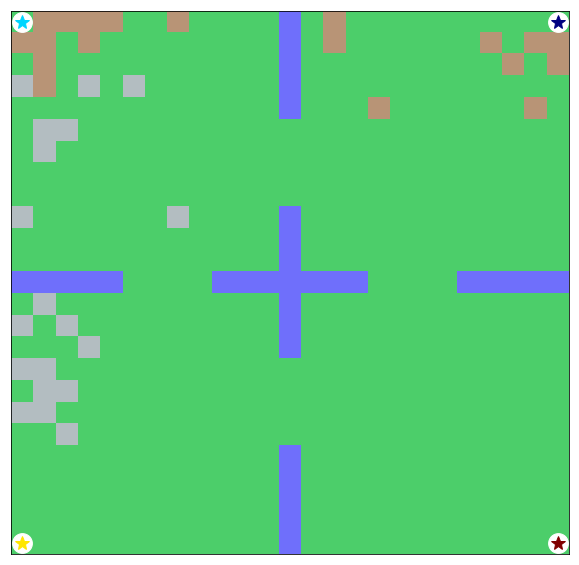
\includegraphics[width=0.5\textwidth]{Resources/imgs/Map_0.png}
    \caption[Rendering of the world at inital conditions: ]%
    {\label{img:map_0}Rendering of the world at inital conditions: \small \textit{this is a rendering of the world map at the first timestep of the simulation, blue blocks are water, brown blocks are wood sources, grey blocks are Stone sources. The four corners are the starting positions for the 4 agents.}}
\end{figure}



\subsection{Game dynamics}

A problem that has a continuous flow of agent-environment interactions can be formalized by a Finite Markov Decision problem \cite{sutton2018reinforcement}. In particular, this simulation is a partial-observable multi-agent Markov Games (MGs). The problem is defined by the tuple \(\left(  S,A,R ,\gamma, o, \mathcal{T} \right) \) where \( S \) is the state space, \( A \) is the action space, \( R \) the reward space and gamma a dicount factor. 

The simulation is composed of a series of episodes, each of length \( H \) time-steps. At every point in time \( t \in [0,H] \) the episode is characterized by a state \( s_t \), representing the current world environment, every agent performs an action \( a_{i,t}  \)  given the current partial observation \( o_{i,t}\) of the world state, and receives a reward \( r_{it}  \). Afterwards the environment transits to a new state \( s_{t+1} \) according to the transition distribution \(  \mathcal{T}(s_{t+1}|s_t,\boldsymbol{a}_t)\). This chain of interactions state-action-reward/state carries on until the end of an episode.

\begin{equation*}
     s_0 \,  \rightarrow_{\boldsymbol{o}_0}\, \boldsymbol{a}_0 \,\rightarrow\, r_1 , s_1 \,\rightarrow_{\boldsymbol{o}_1}\, \boldsymbol{a}_1 \,\rightarrow ... \rightarrow_{\boldsymbol{o}_{H-1}}\, \boldsymbol{a}_{H-1} \,\rightarrow\, r_H , s_H
\end{equation*}

Here \( \boldsymbol{a} \) and \( \boldsymbol{o} \) are the vectorized observations and actions for all the five agents. Given the particular structure of the simulation every single agent will receive an observation at every time-step (different for everyone, more on that later), but only at the 4 basic agents will be asked to act, the policymaker will act only upon a certain condition met. In this case, the episode lasts for 1000 time-step and the policymaker is asked to act (tax the other agents) every other 100 steps. The existence of multiple episodes is necessary for the 4 agents and the policymaker to define their own optimal policy \( \pi_i(o_{i,t}, h_{i,t-1};\theta_i^*) \), this optimization process will be discussed in the RL chapter.

\subsection{Agents}

Fromthe information above we know that the four basic agents are endowed with labor, coins, wood and stone. They live in the world map, can act within it and their objective is to maximize their $\gamma$-discounted utility function. Now I will describe in more detail the agents starting from the information that they receive at each time-step, then talking about the actions that they are allowed to take and finally about their objective. 

\paragraph{Observation space:} Given that this simulation is a partial-observable multi-agent Markov Game, the observation that agent \( i \) receive at time \( t \) is not complete but partial, this information can be summarized in the following way:

\begin{itemize}
    \item \(o_{i,t}^{\text{world state}}\): world map situation surrounding the agent, this is limited to the 11x11 grid around the agent \( i \).
    \item \(o_{i,t}^{\text{market state}}\): full information about the market state for wood, stone and available trades.
    \item \(o_{i,t}^{\text{agent}}\): public resources and coin endowments (this information is also available to the policy maker), private labor performed and skill level.
    \item \( o_{i,t}^{\text{tax}} \): tax structure
    \item \( o_{i,t}^{\text{other}} \): other information (ex. action mask)
\end{itemize}
 
the full observation space can be seen in Table \ref{tab:full_obs}

\paragraph{Action space:} The agent can take one action per time-step and can choose this action from the 50 listed below:

\begin{itemize}
    \item \textbf{Movement}: 4 actions for the basic movements N, S, E, W
    \item \textbf{Gather}: 1 action for gathering resources
    \item \textbf{Trade}: 44 actions for trading resources
    \item \textbf{Idle}: 1 action that does nothing
\end{itemize}

The movement's actions along with gather do not need much of an explanation, these are simple actions that increases labor by 0.21 units each time pursued. The building action requires the agent to consume (destroy) one unit of wood and one unit of Stone, as a consequence he gains 2.1 units of labor and an amount of coin that depends on his skill level. The most complicated set of actions are the one that rules trading. Each one of them is a combination of the 11 price levels [0,1,...,10] that the agent is willing to (pay/request) for each side (bid/ask) and for each resource (wood/stone). A trading open action remains open for 50 turns, if in this time span it is matched by the corresponding counteraction at the same price (a bid for an ask and vice versa) then the trade takes place and each agent gets 0.05 unit of labor.

Furthermore, notice that during the episode agents might incur into a series of inconclusive actions, such as moving north while at the north border of the map or building a house without the required wood and stone. The so called action mask,  present in the observation space, is used in the learning process to avoid wasting time exploring these possibilities. It is an array of binary values of length 50 that "masks" all meaningless actions.

\paragraph{Agent objective}

Agents in the simulation earn coins when building houses or trading goods, the utility for the four agents is an isoelastic utility:

\begin{equation}
u_i(x_{i,t}, l_{i,t}) = crra(x_{i,t}^c) - \vartheta_k l_{i,t}\,, \quad crra(z) = \frac{z^{1- \eta}-1}{1-\eta}\,,\,\, \eta > 0
\end{equation}

Where \( l_{i,t} \) is the cumulative labor associated with the actions taken up to time \( t \), \( x_{i,t}^c \) is the coin endowment and \( \vartheta \) is a function utilized for labor annihilation with the following specification \( \vartheta_k = 1- exp\left(- \frac{\textit{episode completitions}}{\textit{energy warm-up constant (k)}}\right)\). This variable will play an important role during the two-step optimization process purposed in the original paper. In particular, during phase 1 of training, the labor cost is annihilated to help agents avoid sub-optimal behaviors. And \( \eta \) determines the degree of non-linearity of the utility. This utility function is assumed to be the same for all the agents.

The maximization problem is solved for a rational behaving agent by optimizing the total discounted utility over time,


\begin{equation}
\forall i \,:\, \max_{\pi_i}\mathbb{E}_{a_i \sim \pi_i, \boldsymbol{a}_{-i} \sim \boldsymbol{\pi}_{-i}, s^{'}\sim\mathcal{T}}\left[ \sum_{t=1}^H \gamma^t r_{i,t} + u_i({x_{i,0}l_{i,0}})\right]
\label{eq:agent_max}
\end{equation}


with \( r_{i,t} = u_i(x_{i,t},l_{i,t})  - u_i(x_{i,t-1},l_{i,t-1}) \) being the istantaneous reward of agent \( i \) at time \( t \). Equation \ref{eq:agent_max} illustrates a multi-agent optimization problem in which actors optimize their behavior at the same time since the utility of each agent is dependent on the behavior of other agents. Another agent, for example, may deny an agent access to resources, limiting how many houses the agent can create in the future and hence its utility. While computing equilibrium for complicated environments like this is still out of reach, we will see later how RL may be utilized to produce meaningful, emergent behaviors.


\subsection{Policymaker}

The policymaker, or social planner, differs deeply from the previous agents. Being the focus of the research question its structure and behavior change a lot in every single simulation. Due to the complexity of creating a multi-agent neural network with different objectives I was not able to introduce a policymaker that behaves according to an RL algorithm. This makes the policymaker less interesting from a structural point of view but its behavior is still meaningful for the results it produces.

The only observation needed is the number of coins that each agent possesses. With this value is possible to place an agent within a tax bracket and tax it accordingly to some predefined values. 

There will be five simulations in this thesis: 

\begin{itemize}
    \item US taxation
    \item Italian taxation
    \item Free market
    \item Communism
    \item Flat tax
\end{itemize}

and the policymaker will act accordingly to these taxation systems. The US taxation is based on the 2018 US federal tax and brackets, and the Italian is based on the 2020 INPS tax and brackets. The brackets are created in such a way that 1 coin in the simulation is equal to 1000 \$ or \EURcr 863.93  according to the tax system.  